\chapter{Introduction}
\graphicspath{{Chapter01/Figures/}}

Due to the large variety of products and digital content available on the Web, an increasing number of people are interested in obtaining personalized suggestions, in order to reduce the effort of inspecting all the items in a catalog for selecting the best one according to their preferences. An automated tool capable of recommending items to users in a personalized way is defined as a \textit{recommender system}~\cite{Ricci2015}.

Recommender systems (RS) were initially conceived at the beginning of the 1990s~\cite{Goldberg1992} and, nowadays, they are considered part of a research field that is independent from information retrieval~\cite{Herlocker2000}. In fact, while search engines are based on queries and, therefore, they react to user stimuli, recommender systems try to automatically identify items that could be of interest for a certain user~\cite{Balabanovic1997}.

A popular recommendation technique, called collaborative filtering (CF), consists of learning users' preferences by only relying on their interactions with the items available in a catalog. For example, using a nearest-neighbor search or a machine learning model, it is possible to select the most relevant items for each user who has interacted enough with the system~\cite{Su2009}. An alternative approach to this problem is represented by content-based recommenders, which can generate suggestions by matching users' profiles with the features of the items~\cite{Balabanovic1997,Basu1998}. Another family of recommendation methods proposed in the literature is represented by hybrid algorithms that are capable of combining both collaborative and content-based filtering for mitigating the individual weaknesses of the previous techniques~\cite{Stai2016}.

In a collaborative filtering setting, users are typically required to rate items that are already familiar with, relying on a numerical scale, for example a 5-star scale. This value should objectively represent the utility that the user gained from the consumption of that item. Given a sufficient number of users and ratings, a recommender system is capable of predicting the utility score that a user would assign to unrated items~\cite{Adomavicius2005}. The items with the highest predicted rating are finally suggested to the user, in a top-$k$ ranked list.

A well-established line of research is related to the minimization of the error in predicting these values. However, such a task has limited practical applications, because several techniques capable of predicting ratings with a high accuracy are already available~\cite{Park2012}. Furthermore, accurate suggestions may sometimes not be the most useful ones for users~\cite{Herlocker2000}. For example, predicting high ratings for a popular item is probably accurate, but not meaningful, as users are likely to be already aware of that item.

In recent years, this traditional approach has been put aside in favor of others closer to the needs of the users. For example, many recommender systems now rely on binary or implicit signals in order to create a personalized experience~\cite{Gunawardana2015}. Those signals are more intuitive to be understood and easier to be generated. Another important factor that has started to be considered as a possible input of the recommender is the temporal dimension of the preferences~\cite{Quadrana2018}.

In general, the offline evaluation of recommender systems is a challenging task, because, differently from the field of information retrieval, the ground truth is always uncertain, as it is based on the subjective preferences of the users collected before the introduction of the system under evaluation~\cite{Herlocker2004}. In fact, it is widely known that novel recommendation approaches should be evaluated in the context of online experiments involving human subjects in order to obtain reasonably robust results about their performance.

Nevertheless, most of the studies available in literature support their conclusions with offline trails relying on the preferences of users collected without considering the algorithms under investigation~\cite{Gunawardana2015}. Despite the possible weaknesses of this approach~\cite{Said2014}, offline experiments are extremely popular among researchers because of their limited costs and the theoretical reproducibility of their results. In industry, they are usually considered a powerful tool for pruning the number of possible recommender systems that need to be tested with real users, thus mitigating the economical impact of eventual failures.

This dissertation discusses how to perform the offline evaluation of a generic recommender system by exploiting a multicriteria approach that relies on a comprehensive set of different metrics. By adopting the proposed protocols, it is possible to obtain a more general picture of the systems under evaluation, avoiding frequent problems like the popularity bias and the non reproducibility of the results. We experiment with multiple offline evaluation techniques in the context of both traditional and sequential recommenders.

Furthermore, we investigate the main characteristics of different rating datasets and how they can influence the performance of the systems that rely on them. Finally, we also consider the topic of multicriteria from a different angle, by analyzing existing methods for exploiting a multifaceted knowledge of users' preferences.

More formally, we answer to the following \added{top-level} research questions.

\begin{description}
\item[RQ1\label{int:itm:rq1}] \added{What is the current state-of-the-art regarding multicriteria recommender systems and how they are evaluated in literature?}
\item[RQ2\label{int:itm:rq2}] \added{How can a multicriteria evaluation approach be exploited for comparing different sequence-based recommender systems?}
\item[RQ3\label{int:itm:rq3}] What is the most suitable protocol for performing an offline evaluation of a top-$k$ recommender system?
\item[RQ4\label{int:itm:rq4}] To what extent the structure of a rating dataset can influence the results of an offline evaluation?
\end{description}

\added{As regards}~\ref{int:itm:rq1}, \added{we conduct a systematic literature review to investigate in depth the field of multicriteria recommender systems, considering the exploited recommendation approaches and how the proposed algorithms were evaluated.}

\added{We analyze the different machine learning and data mining techniques typically exploited in literature and we classify them according to the recommendation phase. Furthermore, we review how the proposed algorithms have been evaluated with respect to the experimental settings, the metrics, and the datasets. In Chapter}~\ref{chap:multicriteria}, \added{we provide detailed answers to the following research questions.}

\begin{description}
\item[RQ1.1] \added{What are the most relevant studies addressing multicriteria RSs?}
\item[RQ1.2] \added{What are the most challenging problems faced by researchers?}
\item[RQ1.3] \added{What are the approaches used by multicriteria recommenders?}
\item[RQ1.4] \added{Which techniques and methods have been proposed?}
\item[RQ1.5] \added{In which domains multicriteria recommender systems are applied?}
\item[RQ1.6] \added{Which protocols and frameworks are used for their evaluation?}
\item[RQ1.7] \added{Which metrics are considered during their evaluation?}
\item[RQ1.8] \added{Which datasets are used for testing the algorithms?}
\item[RQ1.9] \added{What are the most promising directions for future works?}
\end{description}

With respect to~\ref{int:itm:rq2}, we research and prototype an offline evaluation framework called Sequeval that is designed to evaluate recommender systems capable of suggesting sequences of items, instead of lists of items. In Chapter~\ref{chap:sequeval}, we provide a set of mathematical definitions to characterize in a precise way what is a recommender system capable of suggesting sequences. In detail, we expand the traditional concept of rating by adding to it the notion of temporal dimension.

Then, we propose to consider a sequence as a temporally ordered list of ratings and a sequence-based recommender as a function that is able to return a sequence given its required length and a seed rating. These definitions are conceived as an extension of the seminal works on recommenders capable of suggesting sequences available in literature~\cite{Quadrana2018}.

Starting from this formalization, we propose an evaluation protocol that can be applied to any sequence-based recommender system. First, an initial dataset is transformed into a set of sequences. Then, the available sequences are split between training and test sets. At this point, one or more external recommenders are plugged into the framework: they are exposed to the training sequences and they are asked to create suggested sequences starting from the same seeds of the test ones. Finally, considering the recommendations available, the framework can compute eight different evaluation metrics.

We report the lessons learned using this framework for assessing the performance of four baselines and two recommender systems based on conditional random fields and recurrent neural networks, considering two rating datasets. Sequeval is publicly available and it can be exploited by researchers and practitioners when experimenting with sequence-based recommender systems, providing comparable and objective evaluation results. \added{In Chapter~\ref{chap:sequeval}, we consider the following research questions.}

\begin{description}
\item[RQ2.1] \added{What is the formal definition of a sequence-based recommender system?}
\item[RQ2.2] \added{How already established metrics can be extended and adapted for evaluating a sequence-based recommender system?}
\item[RQ2.3] \added{Against which baseline approaches a sequence-based recommender system can be compared?}
\end{description}

For addressing~\ref{int:itm:rq3}, we introduce RecLab, an evaluation toolkit discussed in Chapter~\ref{chap:reclab} and based on RESTful APIs that can be used to overcome the problem of evaluating traditional recommenders in heterogeneous settings. In fact, because the recommenders are deployed on different servers, the evaluator does not need to know their implementation details.

The researcher can specify the experimental parameters in a Web-based interface for starting a new evaluation campaign. RecLab will then contact all the recommenders selected as part of the comparison and it will display the results computed considering a comprehensive set of seven different metrics.

We propose a Web-based interaction protocol in order to standardize the procedure for evaluating the recommenders. The evaluator first requests the training of a new model, then it provides the training set created according to the settings of the experiment. When the model is ready, the evaluator asks the recommender to create a list of $k$ suggestions for each user of the test set. The results of all experiments are permanently stored and publicly available in order to support accountability and comparative analyses. \added{In Chapter~\ref{chap:reclab}, we provide an answer to the following research questions.}

\begin{description}
\item[RQ3.1] \added{How can different top-$k$ recommender systems be fairly compared in heterogeneous settings without necessary exposing their algorithms?}
\item[RQ3.2] \added{To what extent it is possible to support the reproducibility of the experiments and the accountability of the results?}
\item[RQ3.3] \added{How can the availability of different metrics support the experimenter in the interpretation of the obtained results?}
\end{description}

Regarding~\ref{int:itm:rq4}, we explore a method for visualizing the structure of a rating dataset in Chapter~\ref{chap:rs-viz} and we discuss how to generate a synthetic dataset for evaluation purposes in Chapter~\ref{chap:synthetic}.

We introduce a qualitative approach based on data visualization for creating a graphical summary of any collection of user preferences. This method is useful for visually identifying similarities and differences among various rating datasets. In fact, if two datasets result in similar visualizations, the behavior of different recommender systems relying on them will be consistent. Furthermore, we develop a Web-based tool, named RS-viz, for easily constructing the proposed visualization and comparing rating datasets in an intuitive way. \added{In Chapter~\ref{chap:rs-viz}, we consider the following research questions.}

\begin{description}
\item[RQ4.1] \added{How can data visualization techniques be exploited to create a graphical summary of the main characteristics of a rating dataset?}
\item[RQ4.2] \added{To what extent the graphical representation of different rating datasets can be useful to easily identify their similarities and diversities?}
\end{description}

Another relevant problem that we try to address in this dissertation is related to the shortage of publicly available rating datasets. In fact, it is necessary to rely on a collection of user preferences obtained in a particular domain to perform an offline experiment, but the availability of such datasets is often limited. Some researchers have started to rely on synthetic ratings. However, the results obtained from these experiments may be questionable, as the generated datasets are usually not capable of capturing the characteristics of a particular domain of interest.

For this reason, we propose an approach for automatically generating synthetic datasets with a configurable number of users leveraging on a reference dataset that is used as the seed of the process and that encodes the peculiarities of a domain of interest. Such a method could also be exploited for anonymizing existing datasets before their public release in the context of privacy-aware suggestions. \added{In Chapter~\ref{chap:synthetic}, we analyze the following research questions.}

\begin{description}
\item[RQ4.3] \added{What is the impact of using a synthetic dataset instead of a real one on the results of an offline experiment in the context of recommender systems?}
\item[RQ4.4] \added{Can a generative approach be exploited to create a synthetic dataset that exhibits properties similar enough to the ones of a real dataset?}
\item[RQ4.5] \added{To what extent this method can be consistently applied to datasets from different domains and of different sizes?}
\end{description}

\begin{figure}
\centering
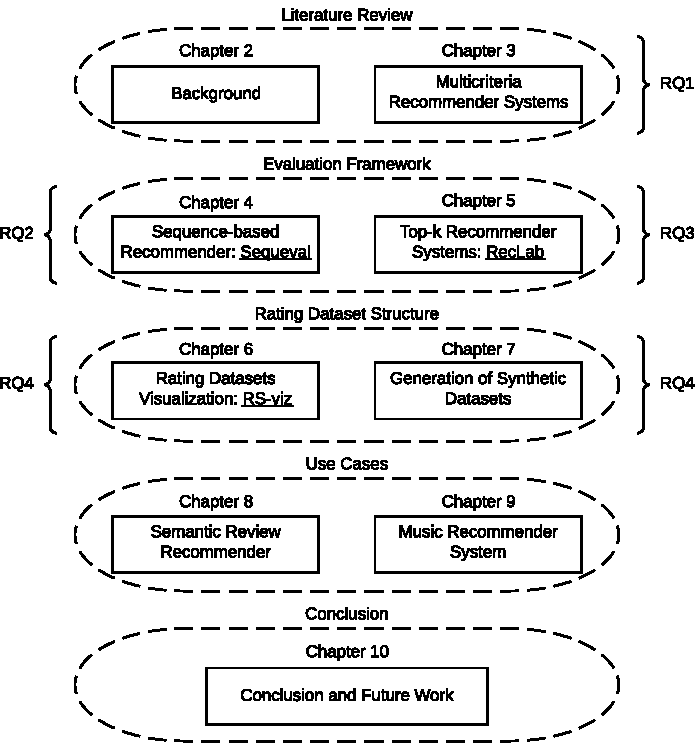
\includegraphics[width=\textwidth]{structure}
\caption[Overview of the dissertation structure]{\added{An overview of the dissertation structure illustrating its division in chapters, the top-level research questions and the main outcomes of the related research activity. The software tools developed are underlined.}}
\label{int:fig:structure}
\end{figure}

In summary, \added{as depicted in Figure~\ref{int:fig:structure},} this dissertation deals with the problem of conducting an offline comparison of recommender systems from different perspectives. We analyze existing approaches for exploiting multicriteria ratings, with a special emphasis on the methods currently employed for validating the quality of the suggestions. Then, we discuss multicriteria evaluation techniques, considering both sequence-based recommenders as well as more traditional approaches. Furthermore, we explore the problem of selecting the right dataset according to the evaluation context by visualizing its structure and generating alternative versions of it. Finally, we apply our knowledge of multicriteria evaluation techniques to different use cases. We propose and evaluate with an ensemble of metrics a semantic review recommender capable of annotating product reviews to extract useful information from them and a music recommender system designed to create playlists starting from a few songs that represent the seeds of the process.

The remainder of this dissertation is organized as follows. In Chapter~\ref{chap:background}, we review existing recommendation and evaluation approaches available in literature and the associated challenges. In Chapter~\ref{chap:multicriteria}, we report the results of a systematic literature review dealing with the topic of multicriteria recommender systems. In Chapter~\ref{chap:sequeval}, we introduce Sequeval, our framework for evaluating sequence-based recommender systems, while, in Chapter~\ref{chap:reclab}, we discuss RecLab, a Web-based evaluation toolkit for top-$k$ recommenders. In Chapter~\ref{chap:rs-viz}, we describe a qualitative method for visualizing the ratings available in any collection of users' preferences. In Chapter~\ref{chap:synthetic}, we present our approach for generating a synthetic dataset that exhibits the same properties of a real one. In Chapter~\ref{chap:semrevrec}, we report on the creation and evaluation of a semantic review recommender, while, in Chapter~\ref{chap:challenge}, we describe our approach for automatically generating music playlists. Finally, in Chapter~\ref{chap:conclusion}, we formulate our conclusions and we discuss open issues and possible future works.
